\documentclass{article}
\usepackage[margin={3cm,3cm}]{geometry}
\usepackage{multicol}
\usepackage[font=small,labelfont=bf]{caption}
\usepackage{graphicx}

\newenvironment{Figure}
               {\par\medskip\noindent\minipage{\linewidth}}
               {\endminipage\par\medskip}


\begin{document}

\title{Large Scale Network Analytics Using Distributed Servers}
\author{Ryan McGrath}
\maketitle

\begin{abstract}

  Analysis of network traffic is necessary for network management and defense. However, analysis of large network traffic captures is difficult due to proportional memory and processing requirements for the quantity of network data. Wireshark, a popular packet analyzer, can have a memory requirement of multiple times its size. This makes it difficult for a single host to analyze multi-gigabyte capture files.  This paper presents a system to divide, distribute, and query large packet captures using a distributed system of lightweight servers. Additionally, an algorithm is demonstrated that decreases the time for additional queries against the same dataset. This system enables network analysis techniques to scale to gigabyte-sized captures.


\end{abstract}


\begin{multicols}{2}
  
\section*{Introduction} % \section* would create section without section
                       % number.


Packet analyzers enable network analysts to examine individual packets.  An analyzer decodes the structure of network protocols encapsulated in the packet and has a filtering syntax to perform queries.  These queries can uncover misconfigured networks, misbehaving users, or even network intrusions. The overwhelming volume of normal traffic makes it difficult to discover limited, infrequent malicious events. This difficulty is compounded as the dataset scales. Packet analyzers have high memory requirements \cite{wireshark} because they reassemble packet sessions and model layers of network protocols.  Other packet analysis tools, such as tcpdump and ngrep, do not create dependencies between packets and filter selected packets in a single pass. While these tools have lower resource requirements, analyzing large datasets can be time-consuming. 

This paper presents a system to analyze large datasets by using a distributed system. The system divides network data among each server, issues commands, collects the results, and balances the amount of data on each server to optimize additional queries. The central server issues commands over SSH and transfers files using rsync to processing servers. The load balancing algorithm adapts for differences in server resource capabilities and data by redistributing the chunks of data from slow to fast processing servers. This improves additional queries against the same dataset. This system enables a distributed system of heterogeneous servers to rapidly divide a large network capture and run queries in parallel. 

The query syntax are tshark, tcpdump, or ngrep commands. Building upon widely used open-source tools enables reuse of optimized packet processing libraries and support for hundreds of protocols. This avoids the complication of translating network data to fit a specific query syntax.  

The system is designed for a variety of use cases. One use case is to develop the query on a subset of the packet capture on a single machine and use the system to run the query against the full dataset.  Another use case is to filter a large dataset to produce output for a consuming analytic. The output can be sent using Unix pipes to tools such as sort, uniq, or count. 

The system could be implemented using a commercial cloud provider to add additional servers until the desired performance is reached. Alternatively, the servers could be laptops that are transported to a client site to function as a tool to support network incident response.

\section*{Related Work}

Several approaches have been developed to analyze traffic and monitor large scale networks. One approach, commonly called netflow \cite{netflow}, is to reduce the size of the captured network data by only storing the metadata. This metadata, such as listing source and destination IP addresses, can be analyzed for anomalies.  This approach requires prior knowledge of what is necessary to capture, and discards most network content. Intrusion Detection Systems (IDS), such as Snort\cite{snort}, take a different approach by scanning traffic for pre-defined signatures. The open source Bro network security monitoring system\cite{bro} combines a netflow approach with IDS-like functionality.  Other efforts, such as pcap2sql\cite{pcap2sql}, translate relevant network events into a database. These approaches enable queries on network data, but are limited by the requirement to know exactly what to extract from network traffic. 

Other efforts have focused specifically on analyzing large network captures using parallel computing. Network traffic has limited dependencies and can be split into parallel workloads for servers to analyze individually.  Techniques from Lee and Lee\cite{lee2013}, and Nagele\cite{ripecc2011} both use a Hadoop-based approach to distribute work among a number of servers.  Lee and Lee's system ingests netflow data and utilizes custom analytics for network statistics while Nagele developed a distributed Domain Name System (DNS) focused analytic and supports structured query language (SQL)-like queries against the captured data.  Both systems require the overhead and complexity of a Hadoop system, translation of the network data to an optimized format, and are tailored for specific analytic uses.  Packetpig\cite{packetpig} is another effort that works on large network captures and utilizes Hadoop to run Apache Pig queries against captured traffic. 

\section*{Methods and Design}

The three primary components of the system are the distribute, command, and load balancing functions. The distribute function splits the packet capture data among the processing servers. The command function executes the packet analysis query on each server.  The load balancing function transfers data between servers to optimize another query against the same dataset.

In the distribute function,  the central server splits the network packet captures into chunks which are distributed equally among the processing servers.  A capture is split into 25 megabyte (MB) chunks. The chunk size is important because the memory requirement can be multiple of the files size on disk. This chunk size was selected because it performed well with the limited resourced Virtual Machines (VM) that were used in development.  Before files are distributed, the central server queries each processing server for files have already been distributed. Then, only files that have changed are transferred.  This allows for efficient repeated queries of a dataset that continues to grow.  All remote communications utilizes SSH public-private key pairs to provide authentication and a secure channel.  The distribution is made using the rsync program running over SSH, and compressed.  Chunks are distributed in a round-robin method among the processing servers so if a single portion of the capture is more complex to analyze, there is a chance that it is distributed equitably among the processing servers.      

In the command function, the central server executes a tshark, ngrep, or tcpdump command on each processing server against the distributed data. The central server uses the user-provided command to construct a bash for-loop that runs on each processing server. An SSH session is established with each processing server concurrently using the python threading library.  Each processing server executes the command against their local allotment of the network data and returns the output and its execution time to the central server. The data is collected from each thread in a thread-safe data structure and sent to standard output in order of completion.

The load balancing algorithm minimizes the disparity in completion times between servers by orchestrating the transfer of data chunks between poorly performing servers and highly performing servers. This lowers the overall task completion time.  The central server records the task completion time for each server.  If the completion time of a processing server is above a user-specified percentage threshold of the average completion time of all servers, the central server marks it as a slow server. If the processing server is below the threshold, it is marked as a fast server.  The central server calculates a number of files to transfer away from the slow server to move that server's completion time closer to the average. The number of transferred files is determined by calculating the average time to processes each file on the slower server. The slow server's completion time is subtracted from the average completion time all servers and then divided by the server's average time per file. This ceiling of this result is the number of files to transfer. The slowest overall server randomly selects files and transfers them to the fastest server.

The process is repeated with the second slowest and fastest servers, and so on, until there is not a pair of servers that performed outside of the threshold.  Transferring files in proportion to the difference from the average completion time moves slower servers quickly towards the average completion time of all servers.  This accomplishes two goals, increased utilization of high capacity servers in a heterogeneous distributed system and leveling the distribution of ''popular'' network data.  An example is if only a small portion of the data was being queried, and this data was concentrated on a single server.  Eventually, the load balancing algorithm will distribute these sought-after chunks among a greater number of servers. The new distribution will decrease the overall task completion time because this data will be analyzed in parallel. 

\section*{Evaluation} 


The objective is to determine the degree of parallelism of the system and specifically to evaluate the efficiency of the load balancing algorithm. The test query extracts all DNS responses out of a 695 MB packet capture. The system is tested with varied number of servers, with and without the load balancing algorithm.  The dataset is split into 26 equal sized chunks, but the time to process each chunk varies.  Since the query only considers DNS traffic, the amount of DNS traffic is the critical factor for execution time as other traffic can be discarded quickly.  Figure 1 shows the relevant statistics of the dataset which was determined by counting the DNS entries per chunk.  There is a large standard deviation between chunks that can cause unequal running times on each processing server.


\begin{Figure}
   \centering
\noindent\makebox[\linewidth]{
\begin{tabular}{llr}
\hline
\multicolumn{2}{c}{Dataset Statistics} \\
\cline{1-2}
Size & 695 MB \\
Data Chunks & 27 \\
Total DNS Responses & 17604 \\
Average DNS Responses per Chunk & 653 \\ 
Standard Deviation & 526.83 \\
Median DNS Responses per Chunk & 419 \\
Max DNS Responses per Chunk & 2393 \\
Min DNS Responses per Chunk & 80 \\
\hline
\end{tabular}
}
\captionof{figure}{Statistics of the dataset relevant to DNS queries.  Note the large standard deviation for number of DNS responses per chunk. The amount of DNS entries is the determining performance factor for a DNS focused query }
\end{Figure}


The tests were conducted using Virtual Machines (VM) allocated 512 MB of RAM and a single core processor. All VMs are hosted on an 8 GB RAM, quad-core Apple iMac. Since resources are reserved for the host operating system, a limited number of VMs can run at once.  Tests with more VMs running can be affected by competition for processor time, disk access, background activity of the host, and the overhead of running the VMs.  This is a limitation to evaluating this system as an ideal evaluation would use a large number of dedicated servers to test the system at scale.

Figure 2 shows the task completion times for ten repeated queries with different numbers of processing servers.  The completion time decreases as the number of servers increases, until more than four servers are used.  After four servers, the overhead out paces any gains from adding more servers to divide the work.  This limit could be the result of of running more than four VMs affected the running time.  Since the host machine has a quad core processor, running more than four VMs could contention on CPU core and increase the completion time. Overall, the load balancing algorithm, represented by the solid, green line, contributed to a decreased completion time for all numbers of servers.

\begin{Figure}
  \centering
  \noindent\makebox[\linewidth]{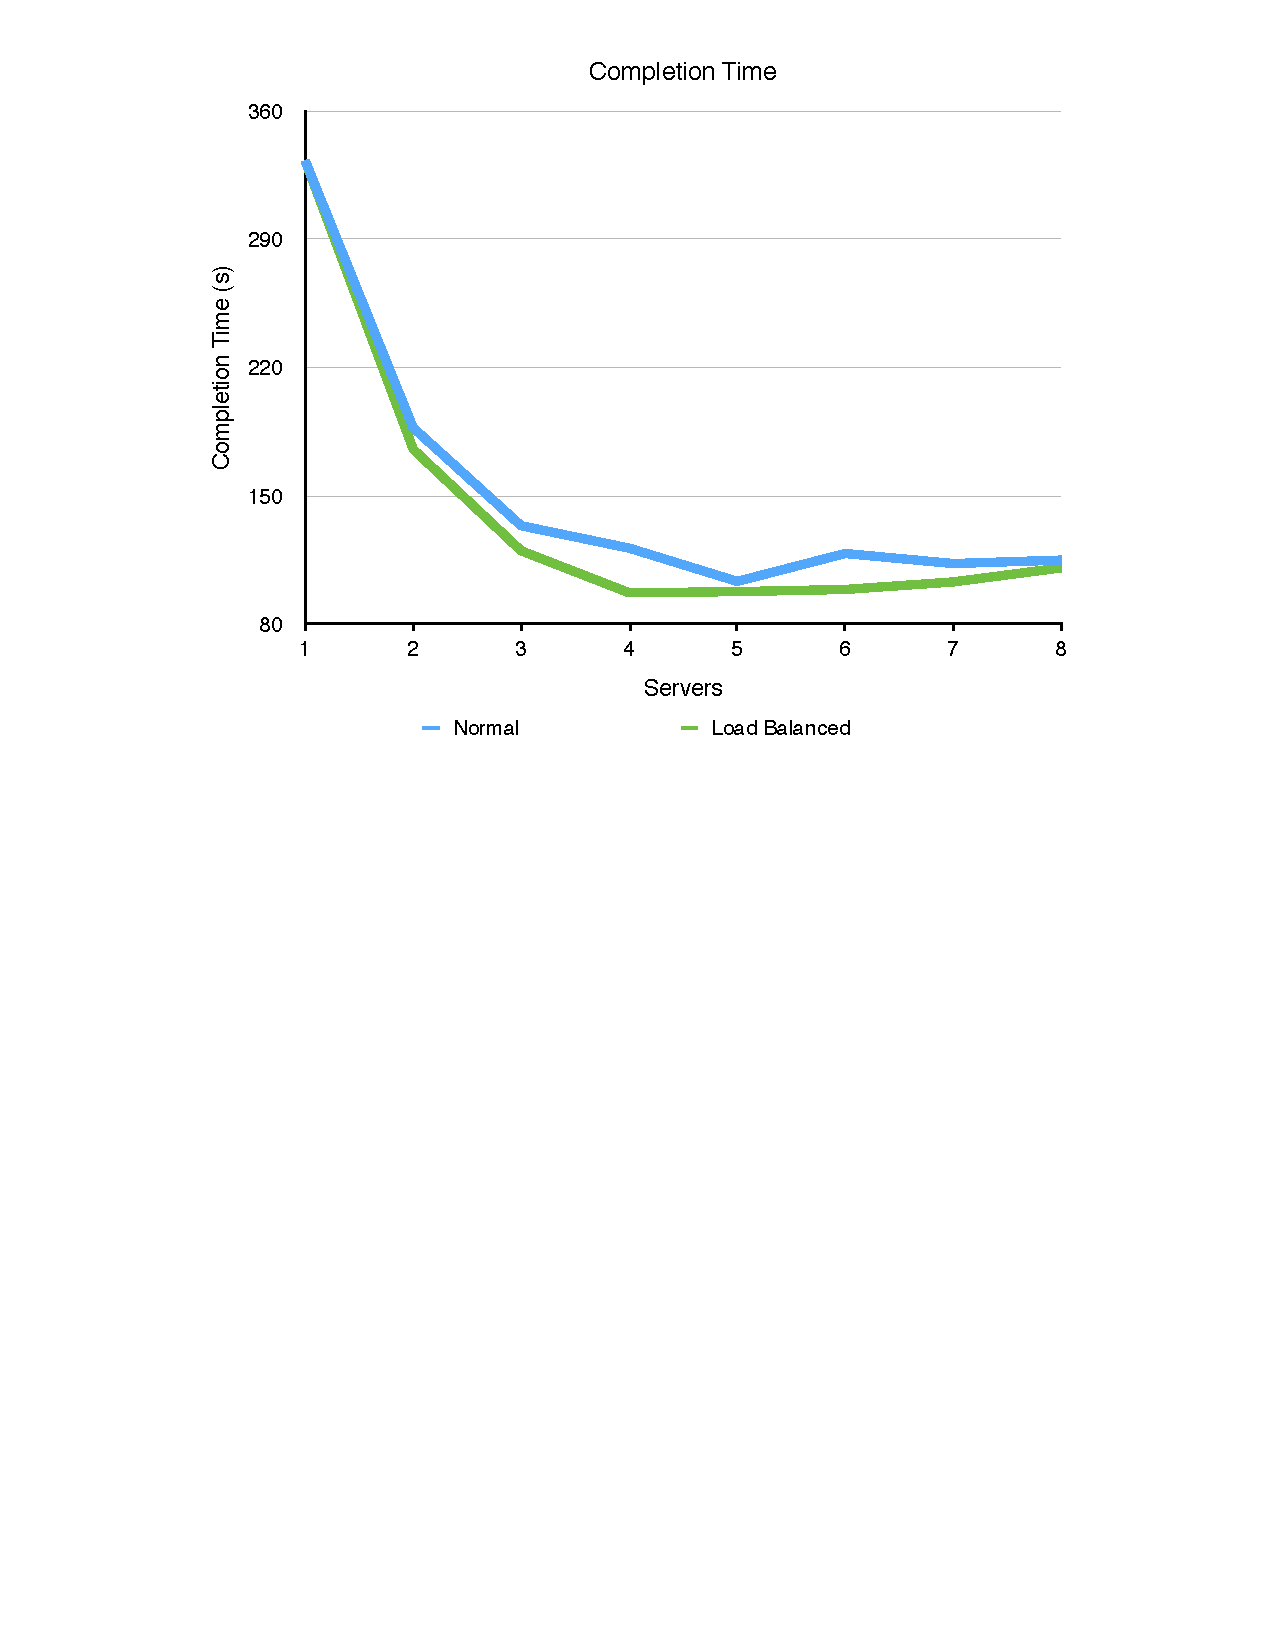
\includegraphics[width=\linewidth]{CompletionTime.pdf}}
  \captionof{figure}{Average task completion time for ten repeated queries as the number of processing servers is increased. The load balancing algorithm lowers the task completion time. More than four processing servers results in a higher task completion time}
\end{Figure}

Examining the performance of four server configuration, Figure 3 shows the difference in completion time when using the load balancing technique.  The blue, broken line, shows the performance of four servers with randomly distributed chunks. The green, solid line, shows the performance when the load balancing algorithm is applied after one query with the random distribution of chunks.  After the first queries there is a marked decrease in completion time which generally persists for repeated queries.  The completion time with load balancing is a 17.1 percent improvement over the average completion time without load balancing.  However, the algorithm can make a data transfer that adversely effects the running time because only the average cost per chunk is calculated rather than knowing the actual cost per chunk. This means an inefficient transfer can be made, but the algorithm will attempt to self correct on the next iteration. Once the threshold is achieved, the algorithm stops data transfers until the threshold is breached.

A possible negative situation for the algorithm would be if a chunk was overwhelmingly computationally expensive, which would cause the algorithm to continuously move this chunk from server to server without reaching the desired threshold.  While this situation was not encountered during testing, a smaller chunk size would split this computationally expensive data and then it could be effectively distributed across servers by the load balancing algorithm. 

\begin{Figure}
  \centering
  \noindent\makebox[\linewidth]{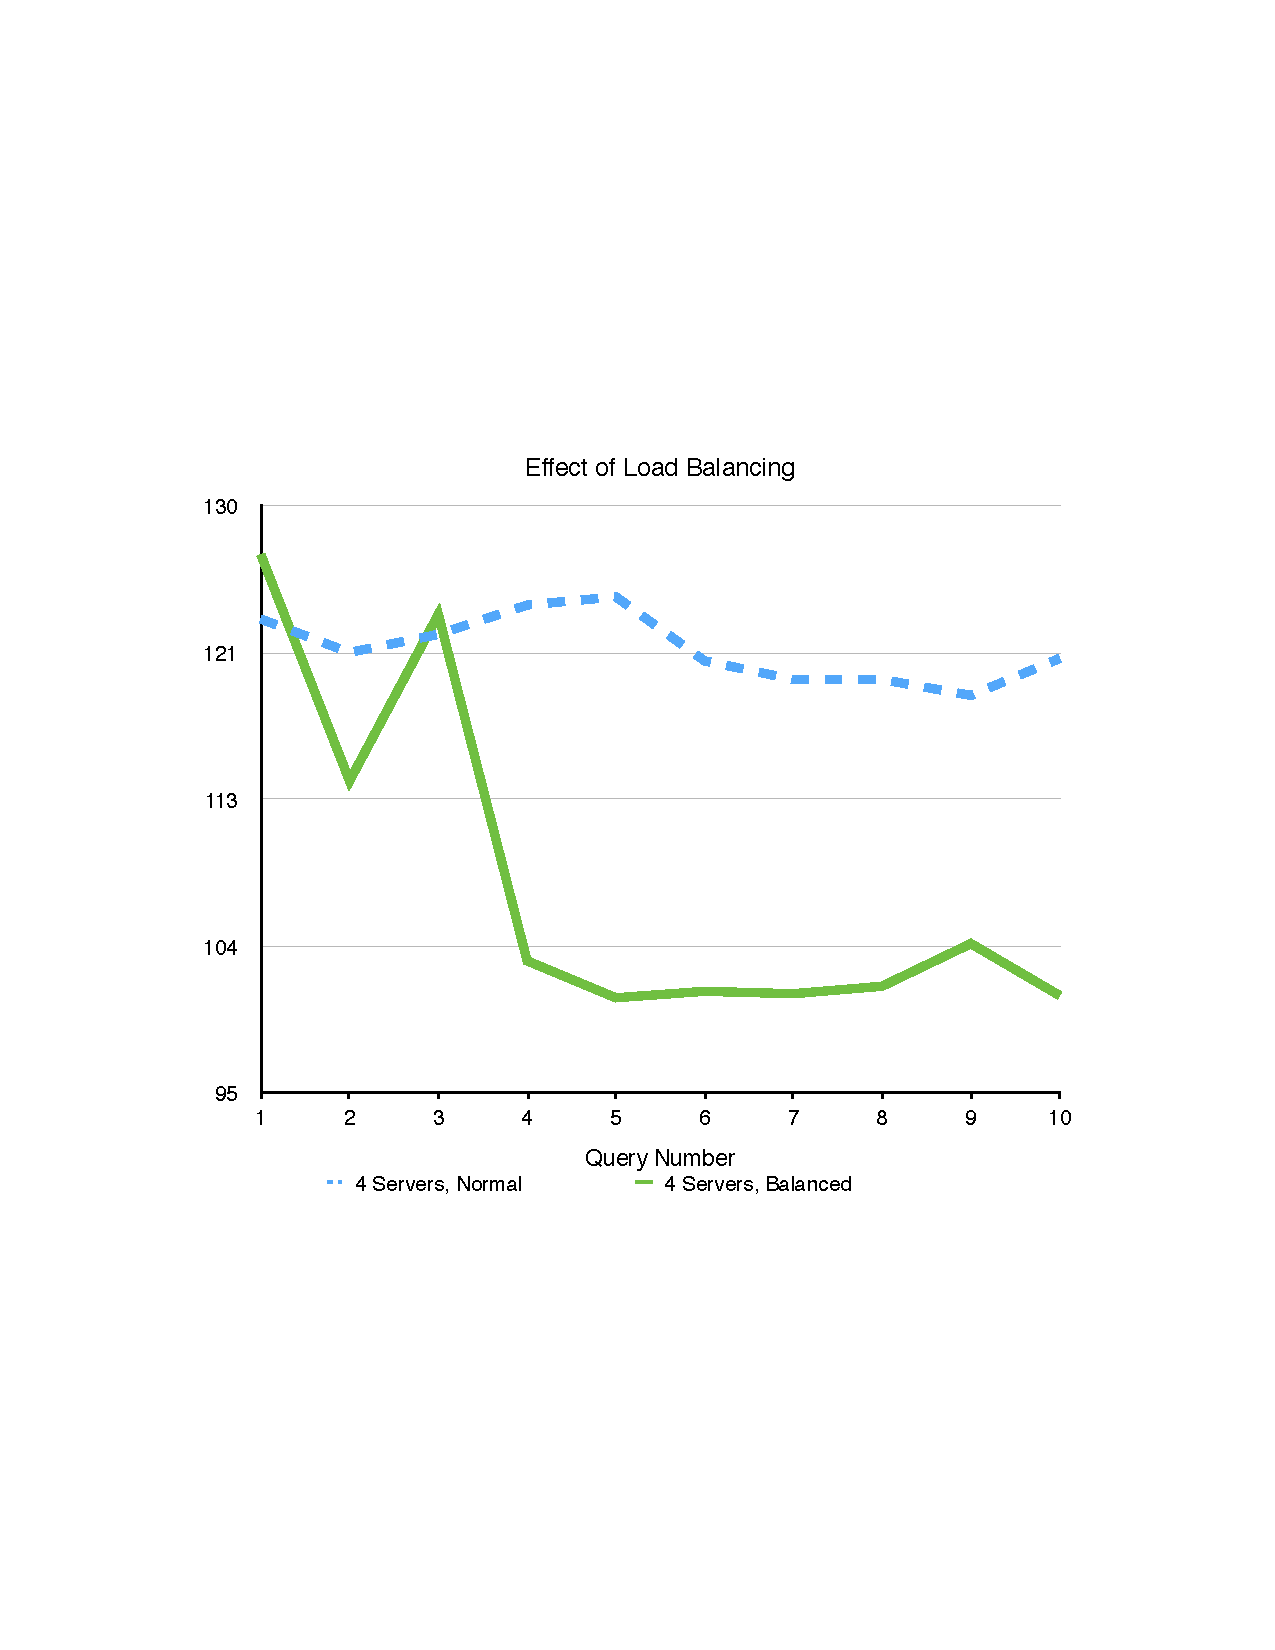
\includegraphics[width=\linewidth]{LoadBalancingEffect.pdf}}
  \captionof{figure}{The completion time peaks at query three because the algorithm made a poor transfer of data after query two.  The algorithm corrects by making a beneficial swap, and the completion time drops below the threshold for the rest of the queries.}
\end{Figure}


Another measurement of the load balancing algorithm is seen in Figure 4, the standard deviation of the individual server completion times when using four servers over 10 repeated queries.  Without load balancing, there is a relatively constant high standard deviation.  The effectiveness of the load balancing is seen in the eventual reduction of the standard deviation.   This reduction results in a lower overall task completion time as shown in Figure 3.   

\begin{Figure}
  \centering
  \noindent\makebox[\linewidth]{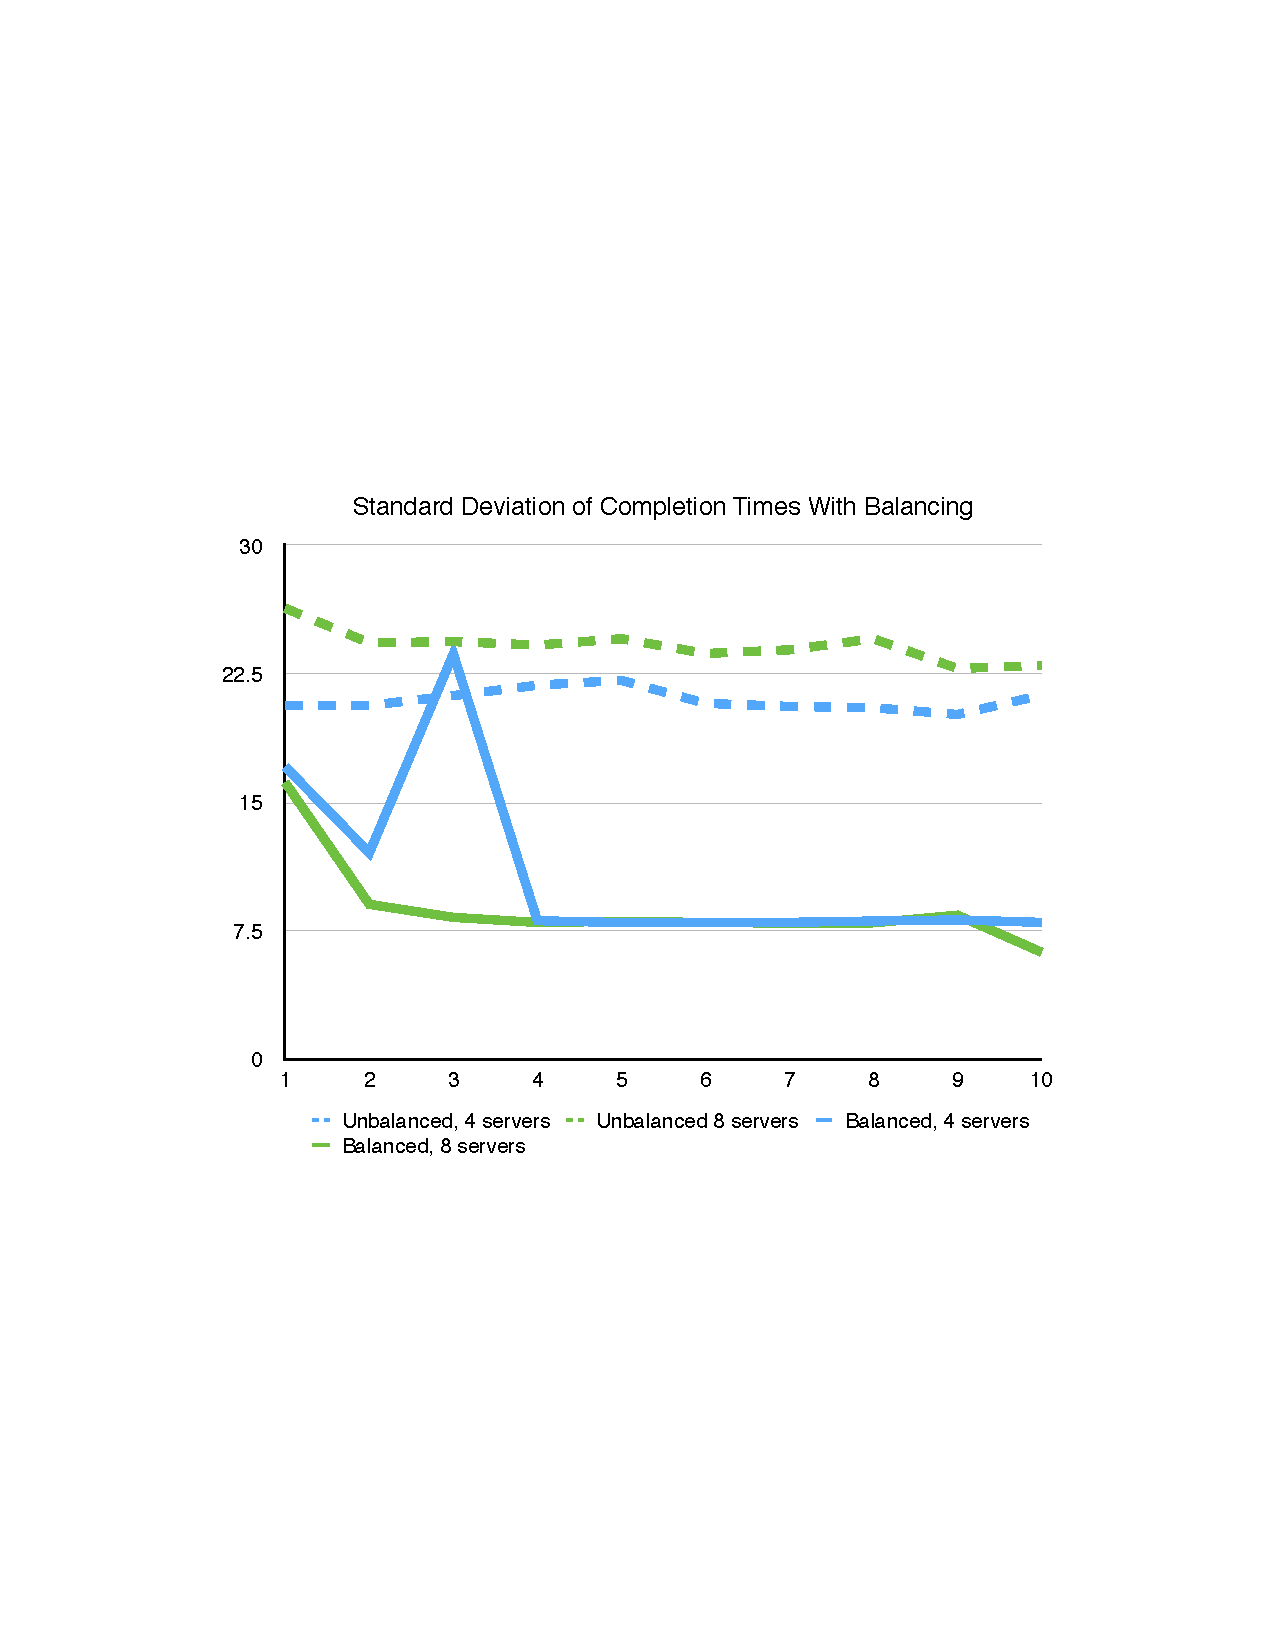
\includegraphics[width=\linewidth]{StandardDeviation.pdf}}
  \captionof{figure}{This is a measure of the standard deviation of the same series of queries as Figure 3.  Note the similarity between the standard deviation of the server completion times and the overall task completion time. As in Figure 3, the standard deviation suffered from the poor transfer of data after query two and benefited from the correction after query three.}
\end{Figure}

When adding additional processing capacity to a distributed system, the best performance is considered ''linear speedup''.  This means that as the number of processing servers is doubled, the speedup would double. Speedup is defined as the execution time for a single server to complete the task divided by the execution time for the multiple server configuration.  For this system there is a less than linear speedup, and loss of improved performance after four servers.  Figure 5 shows a table of the speedup and efficiency results.  Efficiency is a metric that represents the utilization percentage of each server by diving the speedup factor by the number of servers.  An efficiency of 1 would indicate perfect speedup.

\begin{Figure}
   \centering
\noindent\makebox[\linewidth]{
\begin{tabular}{cllll}
\multicolumn{5}{c}{} \\
\cline{1-5}
    & Speedup &  & Efficiency &  \\
\hline
Servers & Normal & Balanced & Normal & Balanced \\
\hline
1&1&1&1&1 \\
2&1.78&1.98&.89&.99 \\
3&2.49&2.79&.83&.93 \\
4&2.74&3.09&.70&.86 \\ 
5&3.22&3.40&.64&.68 \\
6&2.80&3.36&.47&.56 \\
7&2.94&3.23&.42&.46 \\
8&2.89&2.94&.36&.37 \\
\hline
\end{tabular}
}
\captionof{figure}{Table of speedup and efficiency averages for ten repeated queries as the number of processing servers is increased. The load balancing algorithm is an improvement over the randomly distributed data. }
\end{Figure}

Figure 6 shows the efficiency per server as the number of servers increases.  The blue, broken line shows the efficiency of the system with a random distribution of data to the servers, while the green, solid line represents the increased efficiency when using the load balancing algorithm.  The load balancing algorithm increased the efficiency of the system over a random distribution of data.

\begin{Figure}
  \centering
  \noindent\makebox[\linewidth]{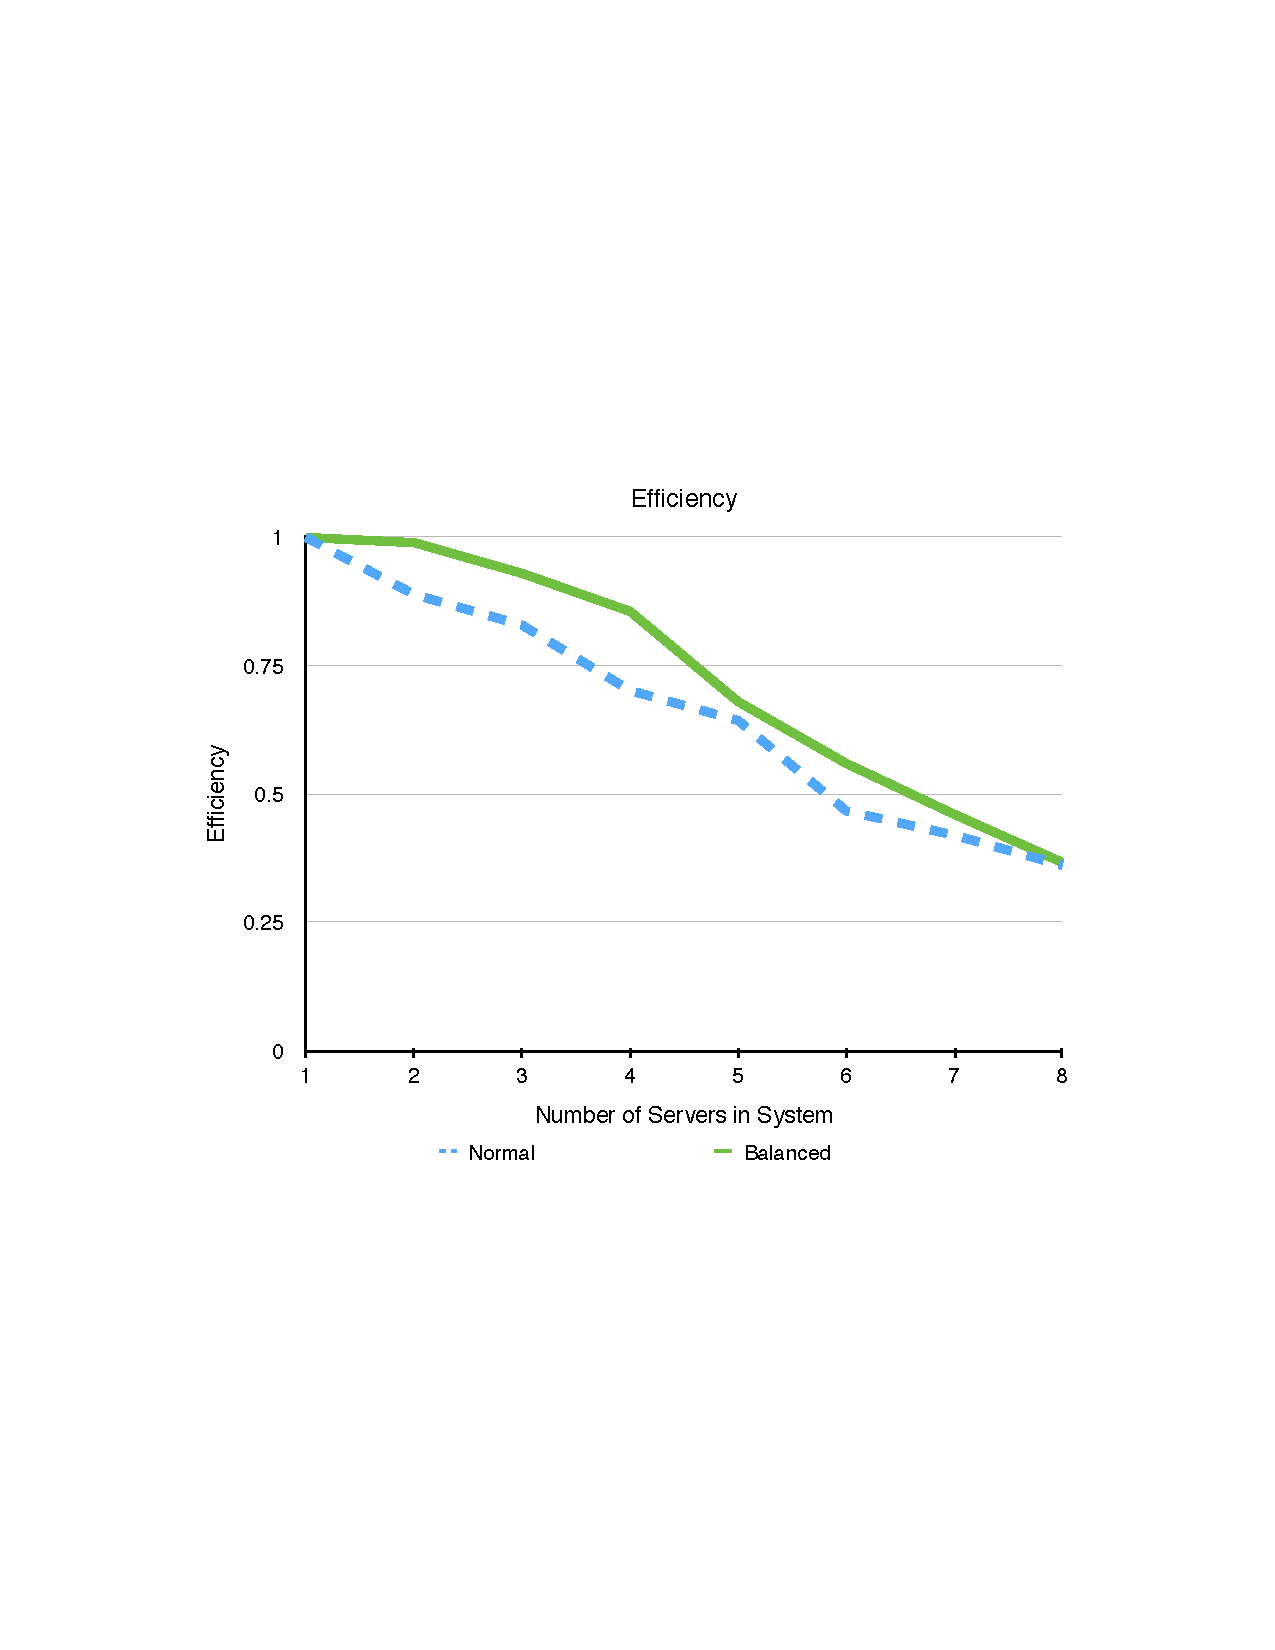
\includegraphics[width=\linewidth]{Efficiency.pdf}}
  \captionof{figure}{Average efficiency per server as the number of servers scale.  With two servers, the efficiency is high and both are fully utilized. With a high number of servers, the efficiency is low as overhead factors limit utilization}
\end{Figure}


There are limitations of this system that were not addressed in this effort.  As the system scales, the central server could become overwhelmed with network traffic as it becomes a hot spot with all communication leaving and returning to it. One extension could have servers assisting with data transfer in a peer-to-peer arrangement instead all transfers originating with the central server.  Another improvement would be to accommodate server failures. One approach would be to track the files that were on the failed server and to re-distributed them to a functioning server.  Another issue is the possibility that the central server could be overwhelmed by a large amount of results. The result of a query could overflow the bounded buffer that is transferring the result back to the central server.   


\section*{Conclusion}
This paper presented a method to process large network captures by parallelizing the analysis.  The load balancing algorithm improved the performance of making additional queries on the same dataset. In spite of the testing hardware limitations the results provide encouragement that this system would scale with dedicated servers and larger datasets. This system analyzed a large network packet capture that would be problematic for a single host. The load balancing algorithm increased the performance of repeated queries.  This system provides the ability to scale intensive network analysis techniques previously only suitable for small packet captures to large ones.



\end{multicols}


\begin{thebibliography}{9}

\bibitem{wireshark}
  Wireshark.
  Wireshark Known Bugs, Out of Memory,
  https://wiki.wireshark.org/KnownBugs/OutOfMemory
  [Accessed: May 10, 2015].

\bibitem{netflow}
  Cisco NetFlow,
  http://www.cisco.com/web/go/netflow.
  [Accessed: May 10, 2015].
  
\bibitem{snort}
  Green, C. and Roesch, M.
  2014.
  Snort Users Manual,
  http://manual.snort.org/
  [Accessed: May 10, 2015].

\bibitem{bro}
  The Bro Project
  2015.
  Bro Manual,
  https://www.bro.org/sphinx/index.html
  [Accessed: May 10, 2015].

\bibitem{pcap2sql}
  pcap2sql
  https://code.google.com/p/pcap2sql/
  [Accessed: May 10, 2015].
  
\bibitem{lee2013}
  Lee, Y. and Lee, Y.
  Toward Scalable Internet Traffic Measurement and Analysis with Hadoop,
  \emph{ACM SIGCOMM Computer Communication Review},
  43, 1, 2013.

\bibitem{ripecc2011}
  Nagele, W.
  2011.
  Large-scale PCAP Data Analysis Using Apache Hadoop. 
  https://labs.ripe.net/Members/wnagele/large-scale-pcap-data-analysis-using-apache-hadoop,
  [Accessed: May 10, 2015].
  
\bibitem{packetpig}
  Baker, M.
  2012.
  Big Data Security Part One: Introducing PacketPig
  http://hortonworks.com/blog/big-data-security-part-one-introducing-packetpig/,
  [Accessed: May 10, 2015].
  
\end{thebibliography}



\end{document}

%%  LocalWords:  Cisco NetFlow Roesch bro packetpig PacketPig
